% The two authors of the 1962 paper.
%
% Both photographs are used under free licences that require attribution, and
% the credit line in the caption is what satisfies that requirement. Do not
% strip it. Licence details:
%   left  -- CC BY 3.0,       Monroe Newborn, Computer History Museum
%   right -- CC BY-SA 2.0 DE, Konrad Jacobs,  Oberwolfach Photo Collection
%
% The two originals have different aspect ratios, so both are set to a common
% height rather than a common width, which keeps the pair visually level.
\begin{tikzpicture}[x = 1mm, y = 1mm]

  \node[inner sep = 0pt, draw = rfaint, line width = 0.4pt] (av) at (0, 0)
    {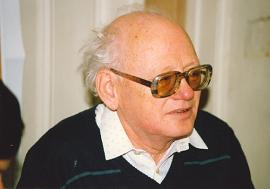
\includegraphics[height = 38mm]{figures/img/adelson-velsky.jpg}};
  \node[tannot, below = 2mm of av.south, anchor = north, align = center]
    {Georgy M. Adelson-Velsky\\[-1pt] \footnotesize (1922--2014), Moscow, 1980};

  \node[inner sep = 0pt, draw = rfaint, line width = 0.4pt,
        right = 14mm of av.east, anchor = west] (la)
    {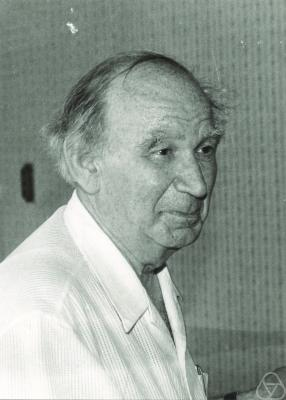
\includegraphics[height = 38mm]{figures/img/landis.jpg}};
  \node[tannot, below = 2mm of la.south, anchor = north, align = center]
    {Evgenii M. Landis\\[-1pt] \footnotesize (1921--1997)};

\end{tikzpicture}
